\documentclass[11pt]{article}
\usepackage{setspace}
\setstretch{1}
\usepackage{amsmath,amssymb, amsthm}
\usepackage{graphicx}
\usepackage{bm}
\usepackage[hang, flushmargin]{footmisc}
\usepackage[colorlinks=true]{hyperref}
\usepackage[nameinlink]{cleveref}
\usepackage{footnotebackref}
\usepackage{url}
\usepackage{listings}
\usepackage[most]{tcolorbox}
\usepackage{inconsolata}
\usepackage[papersize={8.5in,11in}, margin=1in]{geometry}
\usepackage{float}
\usepackage{caption}
\usepackage{esint}
\usepackage{url}
\usepackage{enumitem}
\usepackage{subfig}
\usepackage{wasysym}
\newcommand{\ilc}{\texttt}
\usepackage{etoolbox}
\usepackage{algorithm}
% \usepackage{algorithmic}
\usepackage[noend]{algpseudocode}
\usepackage{tikz}
\usetikzlibrary{matrix,positioning,arrows.meta,arrows}
\patchcmd{\thebibliography}{\section*{\refname}}{}{}{}

\providecommand{\myceil}[1]{\left \lceil #1 \right \rceil }
\providecommand{\myfloor}[1]{\left \lfloor #1 \right \rfloor }


\begin{document}



\title{\textbf{CSDS 455: Homework 3}}

\author{Shaochen (Henry) ZHONG, \ilc{sxz517}}
\date{Due and submitted on 09/02/2020 \\ CSDS 455, Dr. Connamacher}
\maketitle

\section{Problem 1}


\begin{proof}
To prove by induction:\newline

Due to the given $|S| \leq |N(S)|$, there must be $|A| \leq |B|$. Since we know there is a free vertex $a \in A$ and $\myfloor{|B|} = |A|$, we know that there must be at least a free vertex in $B$. It is because if all vertices in $B$ are matched, all vertices must be matched in $A$ as well -- which is a contradiction to the exsistence of $a$. We denote the set of free vertex(ies) in $B$ as $F_b$.

We also know that some free vertex $b \in B$ is connected to at least a vertex in $A$. This is because if we take all matched vertices in $A$ (denote as $M_A$) plus a free vertex $a \in A$ as $S$, we should have at least $|M_A| + 1$ vertices in $B$ connected to this $S$. Since there are only $|M_A|$ matched vertices in $B$, there must be a free vertex $b$ connected to at least a vertex in $A$, we denote this vertex in $A$ as $A_k$.\newline

% For any bipartite graph $G$ with partition sets of $A$ and $B$, a matching $M$, a free vertex set $F_a \subseteq A$, a free vertex set $F_b \subseteq B$, and the $|S| \leq |N(S)|$ relationship as stipulated by the problem; we know that some $b \in F_b$ must be connected to a vertex in $A$, we denote this vertex in $A$ as $P_A$.\newline

If $A_k$ is a free vertex, edge $<A_k, b>$ will be a single-edge argumenting path connecting two free vertex. We then set $A_k$ to be $a$, the statement is trivially proven as an argumenting path from $a$ is found.

However, if $A_k$ is matched vertex (to $B_k$), and there is no single-edge argumenting path in $G$ (otherwise the statement is instantly proven), then we will have the following diagram:

\begin{figure}[H]
    \centering
    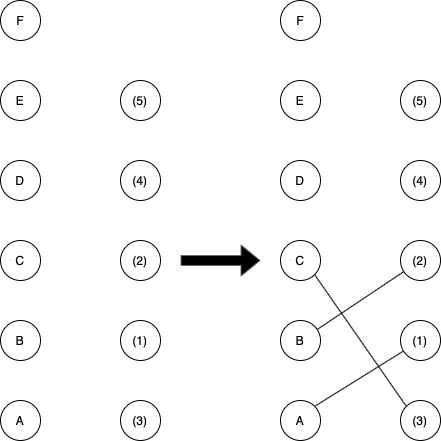
\includegraphics[width=0.7\linewidth]{{fig/fig_1.png}}
    \caption{Structure of $G$ without any single-edge argumenting path}
    \label{fig:1}
\end{figure}

With $B_k$ being the matched vertex connected to $A_k$, we inspect the longest alternating path $P_{k-1}$ starting from $a$. Assume we reached a matched vertex $A_{k-1} \in A$ as a stopping point of $P_{k-1}$. We will try to show that $A_{k-1}$ must connect to $B_k$. Note we delete matched edges that are isolated to the rest of the graph, like matched edge $<A_o, B_o>$ where both $A_o \in A$ and $B_o \in B$ have a degree of $1$; as they will never be part of an argumenting path, nor have any effect on any potential argumenting pathes.\newline

Inspect a path $P_1$ from $a$ to $A_1$, we know that $A_1$ must be conncted to a vertex in $B$. This is because $|P_1 \cap A| = 2$, but $P_1 \cap A$ is only conncted with $1$ vertex $\in B$ ($B_1$). This means at least a vertex in $P_1 \cap A$ must have connected with a vertext $\in B$ other than $B_1$, we denote this vertex as $A_T$.
\begin{itemize}
    \item If $A_T$ is free vertex and is conncted to a free vertex $B_T \in B$, we have a single-edge argumenting path $<a, B_T>$ and the statement is solved. This case is avoided in setup since it is trivial.
    \item If $A_T$ is a matched vertex and conncted to a free vertex $B_T \in B$, we have a argumenting path of $<a, ..., A_T, B_T>$ (in this case, $<a, B_1, A_1, B_T >$). The statement is proven.
    \item If $A_T$ is a matched vertex and conncted to a matched vertex $B_T \in B$, we let this $B_T$ be $B_2$, connect this $<B_T, B_2>$ with an unmatched edge and continuing the induction.
\end{itemize}

We showed that for an alternating path $P_1$ starting from $a$ and stops on $A_1$, we must either be able to find an argumenting path upon this $P_1$, \textbf{OR} $P_1$ can be extended by connecting to a matched node in $B$ but not in $P_1$. Assume it is also true for $P_{k-1}$, and say there are only $k$ matched edges in $M$ (isolated matched edges excluded).\newline


We know that this alternating path $P_{k-1}$ has traversed $k$ vertices in $A$, but due to $a$ is connected to a matched vertex in $B$ (as otherwise we have a single-edge argumenting path direcly), there are only $k-1$ vertices in $P_{k-1} \cap B$. By making this $P_{k-1} \cap A$ as $S$, there must be at least $k$ vertices conncted to this $S$ -- which means there must be a vertex in $P_{k-1} \cap A$ that is conncted to some other vertex in $B$ that are not in $P_{k-1} \cap B$, we again denote this vertex as $A_T$.

The first two cases are essentially same as above, that we can find an argumenting path upon this $P_{k-1}$. The interesting part is in case of $A_T$ being a matched vertex conncted to a matched vertex in $B$, but not in $P_{k-1} \cap B$. Since there are only $k$ non-isolated matched edge in $G$, this $A_T$ can only connect to $B_k$ with an unmatched edge. Since we have a \ilc{matched - unmatched} path on $<B_k, A_k, b$, by connecting this $P_{k-1}$ to $B_k$ with an unmatched graph, we have an argumenting path of $<a, B_1, A_1, ..., A_T, B_k, A_k, b$. Since $<a, B_1, A_1, ..., A_T, B_k, A_k>$ is $P_k$, and we must able to build an argumenting path upon $P_k$, the induction logic is maintained. The statement is therefore proven.



%
% For $N = 1$, there are only two possible ways of constructing a $T_1$:
%
% \begin{figure}[H]
%     \centering
%     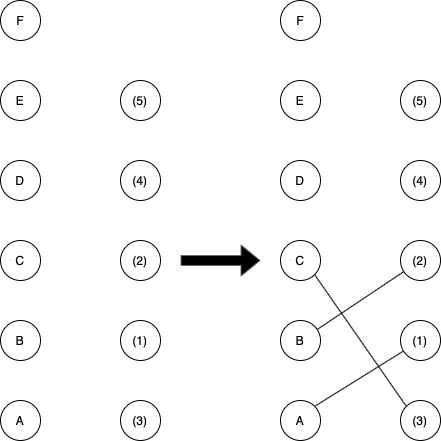
\includegraphics[width=0.5\linewidth]{{fig/fig_1.png}}
%     \caption{Two possible $T_1$ structures}
%     \label{fig:1}
% \end{figure}
%
% Clearly we may locate an argumenting path from both structures, therefore $T_1$ is true. We assume $T_K$ is true for induction. Note that by adding edge(s) to graphs from $T_K$, we can essentially construct all possible graphs. Since the four things we may do to a bipartite graph are:
%
% \begin{itemize}
%     \item Add unmatched edge between two exsisting vertices.
%     \item Change matching (but keep the cardinality of matching to be the same).
%     \item Add another matching edge base on exsisting vertices.
%     \item Add another matching with extra vertices.
% \end{itemize}
%
% Case 1 is trivial since if a graph $T_k \in T_K$ already have an argumenting path, it will still have it even with the extra unmatched edge. Case 2 is also trivial since the cardinality of the matching is not changed, so every possible matching with cardinality of $k$ is included in $T_K$ already. Case 3

\end{proof}


% \section{References}
%
% \nocite{*}
% \raggedright
% \bibliography{references.bib}
% \bibliographystyle{plain}


\end{document}